\documentclass[11pt]{article}
\usepackage[margin=1in]{geometry}
\usepackage{amsmath,amssymb}
\usepackage{graphicx}
\usepackage{booktabs}
\usepackage{float}
\usepackage{listings}
\usepackage{siunitx}
\lstset{basicstyle=\ttfamily\small,breaklines=true}

\title{EE 115 Lab 5\\Frequency Modulation Truncation and Bandwidth}
\author{Kaushik Vada}
\date{\today}

\begin{document}
\maketitle

\section*{Given FM signal}
The passband FM signal is
\begin{equation}
u_{\mathrm{FM}}(t)=\cos\!\left(2\pi f_c t + 2\pi k_f \int_0^t m(\tau)\,d\tau \right)
\end{equation}
with modulation index $\beta=\dfrac{\Delta f_{\max}}{B_m}= \dfrac{k_f\max|m(t)|}{B_m}$. For the single-tone message $m(t)=\cos(2\pi f_m t)$ (so $B_m=f_m$), the complex envelope is
\begin{equation}
u(t)=e^{j\beta\sin(2\pi f_m t)}=\sum_{n=-\infty}^{\infty}J_n(\beta)\,e^{j2\pi f_m n t}
\label{eq:envelope}
\end{equation}
where $J_n(\cdot)$ is the Bessel function of the first kind. Truncating the series to $|n|\le K$ gives
\begin{equation}
u_K(t)=\sum_{n=-K}^{K}J_n(\beta)\,e^{j2\pi f_m n t},
\end{equation}
whose power over one message period is
\begin{equation}
P_{u_K}=J_0^2(\beta)+2\sum_{n=1}^{K}J_n^2(\beta).
\label{eq:power}
\end{equation}
Because $u(t)$ has unit power, $1-P_{u_K}$ is the truncation power error.

\section*{1. Numerical evaluation and plots}
\textbf{Method:} For each $\beta\in\{0.5,\,2,\,5,\,10\}$ and $K=0,\dots,50$, compute $P_{u_K}$ using~\eqref{eq:power}, then $1-P_{u_K}$. Figures~\ref{fig:linear}--\ref{fig:log} show the results on linear and dB scales (dB plotted as $10\log_{10}(1-P_{u_K})$ with a small floor to avoid $\log(0)$).

\begin{figure}[H]
  \centering
  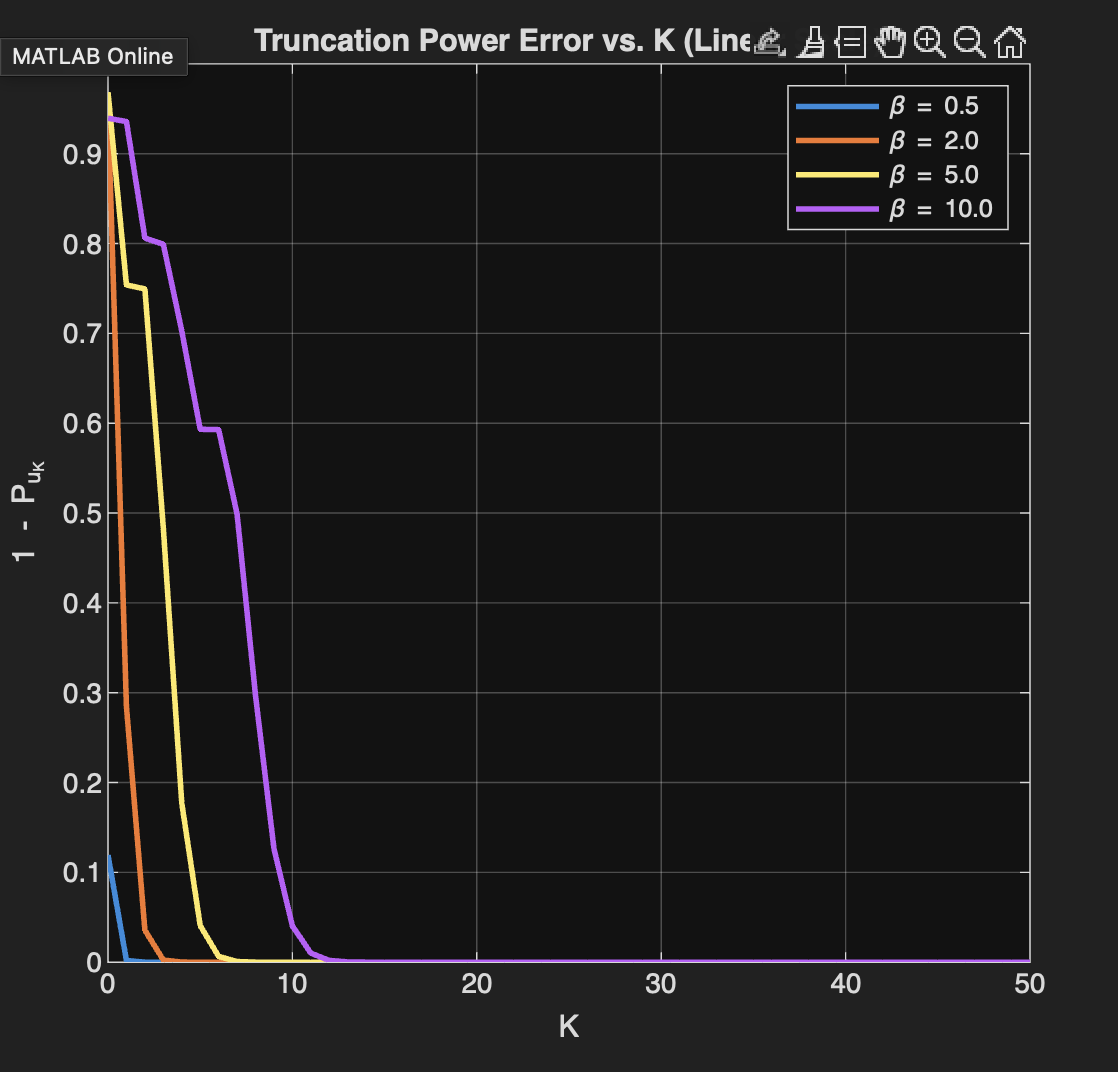
\includegraphics[width=0.9\linewidth]{image1.png}
  \caption{$1-P_{u_K}$ vs. $K$ (linear scale). Higher $\beta$ requires larger $K$ for the same residual error.\label{fig:linear}}
\end{figure}

\begin{figure}[H]
  \centering
  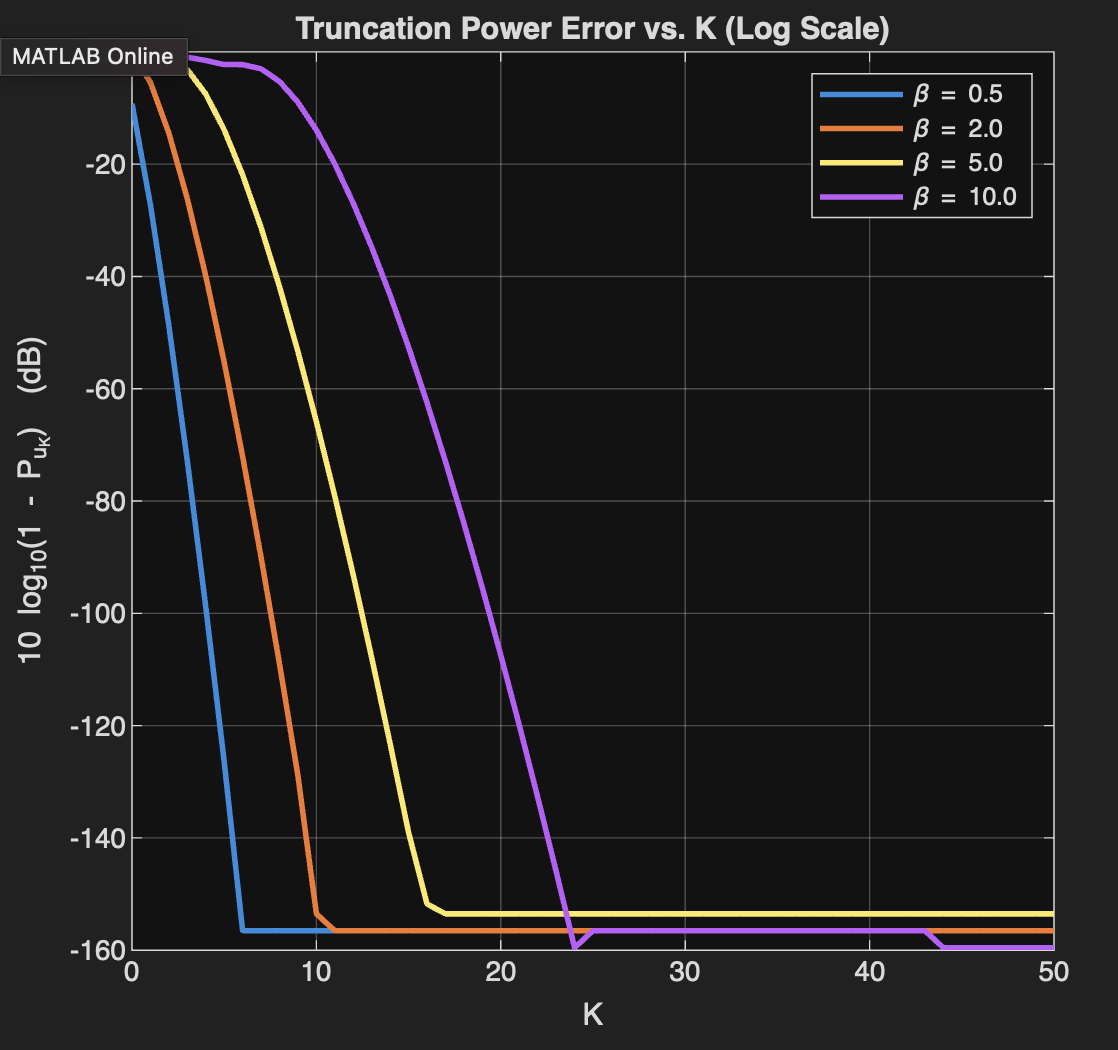
\includegraphics[width=0.9\linewidth]{image2.png}
  \caption{$10\log_{10}(1-P_{u_K})$ vs. $K$ (dB). Residual power falls rapidly once $K\gtrsim\beta+1$, consistent with Carson's rule.\label{fig:log}}
\end{figure}

\textbf{How large must $K$ be?} Using the same computation, the first $K$ that makes $1-P_{u_K}$ drop below several thresholds is:
\begin{center}
\begin{tabular}{@{}lcccc@{}}
\toprule
$\beta$ & $1-P_{u_K}\!\le\!10^{-2}$ & $\le\!10^{-3}$ & $\le\!10^{-6}$ & $\le\!10^{-12}$\\
\midrule
0.5 & 1 & 2 & 3 & 5\\
2.0 & 3 & 4 & 6 & 9\\
5.0 & 6 & 7 & 10 & 14\\
10.0 & 12 & 13 & 16 & 22\\
\bottomrule
\end{tabular}
\end{center}
The table matches the visual takeaway: meaningful coefficients cluster around $n\approx\beta$, and setting $K\approx\beta+1$ captures essentially all the power.

\section*{2. Why $1-P_{u_K}$ is the error power}
Define the truncation error $e(t)=u(t)-u_K(t)$. From~\eqref{eq:envelope},
\begin{equation}
e(t)=\sum_{|n|>K}J_n(\beta)\,e^{j2\pi f_m n t}.
\end{equation}
The complex exponentials $e^{j2\pi f_m n t}$ are orthogonal over any integer multiple of the message period $T_m=1/f_m$, so all cross terms vanish when computing power:
\begin{align}
P_e &= f_m \int_{-1/(2f_m)}^{1/(2f_m)} |e(t)|^2\,dt \\
    &= 2\sum_{n=K+1}^{\infty} J_n^2(\beta) \quad (\text{equal power for } \pm n)\\
    &= 1 - \bigl[J_0^2(\beta)+2\sum_{n=1}^{K}J_n^2(\beta)\bigr] = 1-P_{u_K}.
\end{align}
Because the total power of $u(t)$ is 1, the omitted coefficients account exactly for the residual power. Hence $1-P_{u_K}$ is the power of the truncation error $e(t)$.

\section*{3. Why $B_u \approx f_m(\beta+1)$}
The spectrum of the complex envelope~\eqref{eq:envelope} contains discrete lines spaced by $f_m$ at frequencies $\pm n f_m$ with weights $J_n(\beta)$. For FM, $J_n(\beta)$ is negligible for $|n|>\beta+1$ (the main lobe of $J_n$ sits near $n\approx\beta$ and decays quickly outside that window). Truncating at $|n|\le K\approx\beta+1$ therefore retains essentially all the power, so the one-sided lowpass bandwidth of $u(t)$ is
\[
B_u \approx K f_m \approx f_m(\beta+1).
\]
This matches Carson's rule: the passband FM bandwidth is $W\approx 2(B_m+\Delta f_{\max})=2f_m(\beta+1)$, so the analytic baseband (complex envelope) occupies half that, $B_u\approx f_m(\beta+1)$.

\section*{MATLAB/Octave code (lab\_5.m)}
The following script reproduces the figures and table above.
\begin{lstlisting}[language=Matlab]
% EE 115 Lab 5 - FM truncation error
clear; close all; clc;

betas = [0.5 2 5 10];
Kmax = 50;
K = 0:Kmax;
err = zeros(numel(betas), numel(K));

for idx = 1:numel(betas)
    beta = betas(idx);
    J = besselj(0:Kmax, beta);              % J_n for n = 0..Kmax
    for k = 0:Kmax
        power = J(1)^2 + 2*sum(J(2:k+1).^2);% P_{u_K}
        err(idx, k+1) = 1 - power;          % truncation power error
    end
end

% Linear plot
figure;
hold on; grid on;
colors = lines(numel(betas));
for idx = 1:numel(betas)
    plot(K, err(idx, :), 'LineWidth', 2, 'Color', colors(idx, :));
end
xlabel('K'); ylabel('1 - P_{u_K}');
title('Truncation Power Error vs. K (Linear)');
legend('\beta = 0.5','\beta = 2.0','\beta = 5.0','\beta = 10.0','Location','northeast');
set(gca,'YLim',[0 1]); % keeps the y-axis focused
exportgraphics(gcf,'image1.png','Resolution',300);

% dB plot
figure;
hold on; grid on;
floorVal = eps; % avoid log of zero
for idx = 1:numel(betas)
    plot(K, 10*log10(max(err(idx, :), floorVal)), ...
         'LineWidth', 2, 'Color', colors(idx, :));
end
xlabel('K'); ylabel('10 log_{10}(1 - P_{u_K}) (dB)');
title('Truncation Power Error vs. K (Log Scale)');
legend('\beta = 0.5','\beta = 2.0','\beta = 5.0','\beta = 10.0','Location','northeast');
set(gca,'YLim',[-160 0]);
exportgraphics(gcf,'image2.png','Resolution',300);

% Optional: print thresholds used in the table
thresholds = [1e-2 1e-3 1e-6 1e-12];
fprintf('beta  K(@<=1e-2) K(@<=1e-3) K(@<=1e-6) K(@<=1e-12)\\n');
for idx = 1:numel(betas)
    line = zeros(1, numel(thresholds));
    for t = 1:numel(thresholds)
        kHit = find(err(idx, :) <= thresholds(t), 1) - 1; % zero-based K
        line(t) = kHit;
    end
    fprintf('%4.1f %11d %11d %11d %12d\\n', betas(idx), line);
end
\end{lstlisting}

\end{document}
